\documentclass{article}
\usepackage[margin=3cm]{geometry}
\usepackage{amssymb}

% Figures
\usepackage{graphicx}
\usepackage{color}

% Page formatting
\newsavebox{\notetitle}
\newsavebox{\noteauthor}
\newsavebox{\notenumber}
\newsavebox{\notedate}

\renewcommand{\title}[1]{\sbox{\notetitle}{\begin{minipage}{1.0\textwidth} \begin{center} \Large{\textbf{#1}} \end{center}\end{minipage} }}
\renewcommand{\author}[1]{\sbox{\noteauthor}{\begin{minipage}{1.0\textwidth} \begin{center} \large{#1} \end{center}\end{minipage}}}
\renewcommand{\date}[1]{\sbox{\notedate}{\large{#1}}}
\newcommand{\nb}[1]{\sbox{\notenumber}{\Large{\textbf{#1}}}}

\newcommand{\makemadtitle}{
  \hrule
  \vspace{.5em}
  \noindent
  \begin{center}
  \textbf{
  {\centering
\includegraphics[height=3cm,bb=0 0 371 145]{../fig/logoCHISTERA2014.png}}\\
   {\centering\Large COACHES project, CHIST-ERA 2014 program}
  }
  \end{center}
  \vspace{.5em}
 
  \hrule
  \vspace{3em}
  \begin{center}
    %\begin{large}\textbf{ Note~\usebox{\notenumber}.}\end{large}\\[.5em]
    \begin{Large}\textbf{\usebox{\notetitle}}\end{Large}\\[2em]
    \begin{large}\usebox{\noteauthor}\\ [2em]
    \usebox{\notedate}\end{large}
  \end{center}
  \vspace{3em}
}

% Various macros and environments
\newtheorem{prop}{Proposition}
\newtheorem{proposition}[prop]{Proposition}
\newtheorem{defn}{Definition}
\newtheorem{definition}[defn]{Definition}
\newtheorem{cor}{Corollary}
\newtheorem{corollary}[cor]{Corollary}
\newtheorem{exmp}{Example}
\newtheorem{example}[exmp]{Example}
\newtheorem{lem}{Lemma}
\newtheorem{lemma}[lem]{Lemma}
\newtheorem{fact}{Fact}
\newtheorem{thm}{Theorem}
\newtheorem{theorem}[thm]{Theorem}
\newtheorem{prob}{Problem}
\newtheorem{problem}[prob]{Problem}
\newtheorem{rem}{Remark}
\newtheorem{remark}[rem]{Remark}
\newtheorem{conj}{Conjecture}
\newtheorem{conjecture}[conj]{Conjecture}
\newenvironment{pf}{{\bf Proof }}{\hfill$\Box$\par}
\newenvironment{proof}{{\bf Proof }}{\hfill$\Box$\par}
\newcommand{\spaceafterproof}{\vspace{1em}}

% NOTE ITSELF BELOW %%%%%%%%%%%%%%%%%%%%%%%%%%%%%%%%%%%%%%%%%%%%%

\title{D5.1-Sapienza\\ Definition of internal architecture and interface between software modules}

\author{Roberto Capobianco, Fabio Maria Carlucci, Giorgio Grisetti, Luca Iocchi, \\
Daniele Nardi, and Andrea Pennisi\\
\textit{Dept. of Computer, Control and Management Engineering\\
Sapienza University of Rome\\
via Ariosto, 25 00185 Rome, Italy}}


%\nb{of the kickoff meeting, $27^{th},28^{th}$ October }

\date{Version 2.0 - March 26, 2015}

\begin{document}


\includegraphics[height=3cm]{../fig/logoSapienza.png}

\makemadtitle

\begin{abstract}
This document describes the software architecture of the entire project, showing the main software components, their connections and the interfaces between them.
\end{abstract}

\vspace*{2.0cm}

\fbox{
\begin{minipage}{1.0\textwidth}
\begin{center}
 $\copyright$, THE COACHES CONSORTIUM \\
The copyright in this document is the property of the COACHES Consortium. This document is supplied by the COACHES consortium on the express terms that it is to be treated as confidential. This document is not external distribution without the project manager's permission. 
\end{center}
\end{minipage}
}
\newpage

\begin{figure}
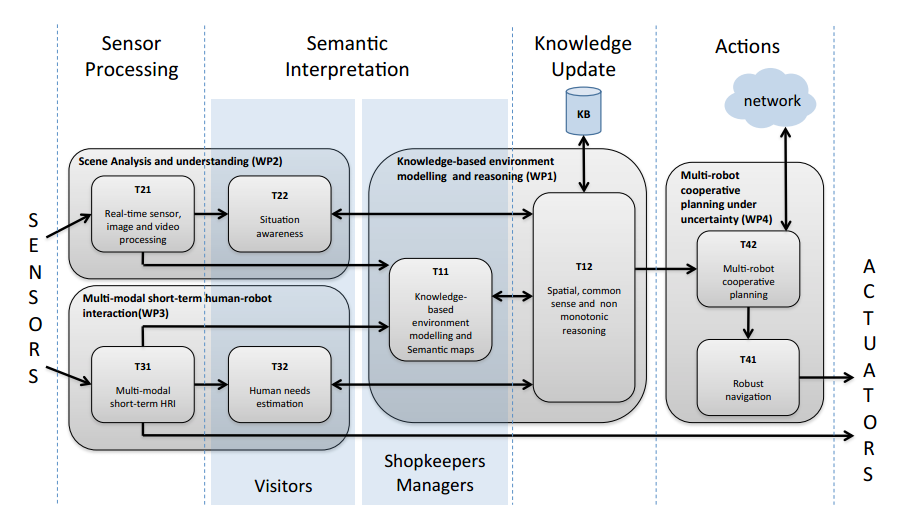
\includegraphics[width=0.95\textwidth]{COACHES_swarch.png}
\caption{COACHES software architecture}
\label{fig:swarch}
\end{figure}

\section{Introduction}

In this document the software architecture developed within the
context of the COACHES project is described.

Design solutions regarding the middleware chosen for implementing the entire system are discussed,
according to the modules shown in Fig. \ref{fig:swarch}).
Subsequent implementation of the software components during the project will follow  these  specifications,  thus  simplifying  their  integration  in  the demonstrators. 
A detailed description of the interface between the modules will be developed at a later stage, where more details on the single components will be provided.


An open architecture (hard/soft) and standard technologies available (such 
as ROS for integrating robotic modules and DDS for communication) will be used,
so that it will be 
easy to extend and/or adapt the capabilities of the system during the whole length of 
the  project  (especially  to  integrate  and  test  various  algorithms  and/or  sensors).  Such 
an open architecture will also simplify and optimize integration efficiency as well as re-use of assets in other projects or products. 

The reminder of this document is organized as follows.
First, the choice of the middleware is discussed, then the main software components and the
set-up of a 2D simulation environment and the collection of data sets for testing the developments are described.
Finally, the version management system that will be used to manage the development is illustrated.

\section{Middleware}

For the development of the software robotics components, the Robot Operating System (ROS)\footnote{www.ros.org}, which is the standard middleware for robotics applications, has been selected.
In particular, the last stable version ROS Indigo and the last LTS (Long Term Support) version 14.04 of the Linux/Ubuntu Operating System will be used.

ROS provides the middleware to share information among the many modules implementing various functionalities on each robot. Moreover, an interface (ROS-through-TCP) will be realized in order to share information among the robots and between each robot and other components of the system.

\section{Main software components}

The main software components that will be developed for control, reasoning and interaction functionalities of the system are listed below.

\begin{itemize}
\item T1.1 KB modeling
\item T1.2 KB reasoning
\item T2.1 Image Processing
\item T2.2 Situation Awareness
\item {\bf T3.1 Multimodal HRI (Sapienza)}
\item T3.2 Human needs estimation
\item {\bf T4.1 Robust navigation (Sapienza)}
\item T4.2 Multi-robot planning
\end{itemize}

Sapienza University is responsible for tasks T3.1 and T4.1 and these tasks are detailed in the next section.

\subsection{Sapienza software components}


Task T3.1 is responsible for bi-directional flows of information between people and robots: automatic speech recognition (ASR), speech synthesis (TTS), graphical user interface in the tablet (GUI). The developed software in this task is distributed in the two laptops of the robots: the tablet laptop, running MS Windows OS, will host ASR and TTS in a multi-language settings (French, English and Italian languagues are envisioned) and the GUI accessible with the touch screen of the tablet. These components are connected with the Linux laptop controlling the robot through a ROS-TCP interface. 
For the human-to-robot interaction, inputs are received from sensors and from the GUI on the tablet, and outputs (i.e., recognized sentences and actions on the GUI) are sent to the knowledge base. 
For the robot-to-human interaction, inputs are received from the low-level actions related to HRI implementing the robot behaviors, while outputs are sent to the hardware devices (speakers and GUI).


Task T4.1 is related to techniques for safe navigation in a populated environment and includes the implementation of both low-level behaviors and the plan generated by the planner module (Task T4.2). 
More specifically, this Task receives as input the plan/policy generated by the planner and it executes it by activating the corresponding actions. More specifically, the policy is transformed  into a Petri Net Plan (PNP) that is then executed by the PNP executor. The PNP executor is also responsible for monitoring the execution of the plan and to report the status of the execution (success, failure, or progress) to the KB component.


Safety is of course of utmost importance in the project and thus in this task we have defined and will implement different levels of security for the COACHES robots as described in the next section.


\subsection{Safety}


\begin{enumerate}
\item Hardware Emergency Stop button. Each robot is provided with two easy-to-access emergency stop button that will immediately cut current to motors in order to stop it.
\item Software Remote Emergency Stop. A wireless device (e.g., a wireless joystick) is configured to disable motor commands immediately, upon pushing a button, in the low-level software module.
\item Obstacle avoidance module. A software module using artificial potential fields for obstacle avoidance is always active.
\item Protection from hardware and software failures. All the low-level software modules are configured in order to immediately stop sending commands to the robot, if they detect any anomaly, such as a sensor not sending data or another software module not working properly. 
\end{enumerate}


\section{Interfaces between software components}

The main interfaces between the modules developed by Sapienza University and other modules in the system are the information collected through human-robot interaction (T3.1) to be used for the semantic map in Task T1.1 and the policy generated by the multi-robotplanner task (T4.2) to be executed in T4.1.

The semantic map of the environment is formed by two components: a metric map, a set of semantic annotations related to the metric map, and a topological map. The semantic annotations includes a taxonomy of the concepts used to describe the environment and a set of instance signatures related to the specific locations and objects in the environment.
A detailed description of the semantic map representation is given in Deliverable \emph{D1.1}.

The policy is a function mapping states to actions representing the desired behavior of the robot. The policy is represented as a set of pairs (state, actions), an initial state and a description of the goal. It is generated by the planner system and used by the execution system in T4.1 to generate a PNP that is ten executed.
More details are given in Deliverable \emph{D4.1}.



\section{2D Simulation Environment}

The simulation environment is based on 2D Stage simulator, which is integrated in the ROS infrastructure. The choice of a 2D simulator (instead of a 3D one) is motivated by: 1) the need of modeling and testing high-level behaviors of the robot that does not involve 3D perception, 2) the possibility of using the simulator for multiple robots and other moving elements representing people in the environment, 3) the possibility of using the simulator on standard laptop, thus not requiring advanced graphical cards for running 3D simulations.

\begin{figure}
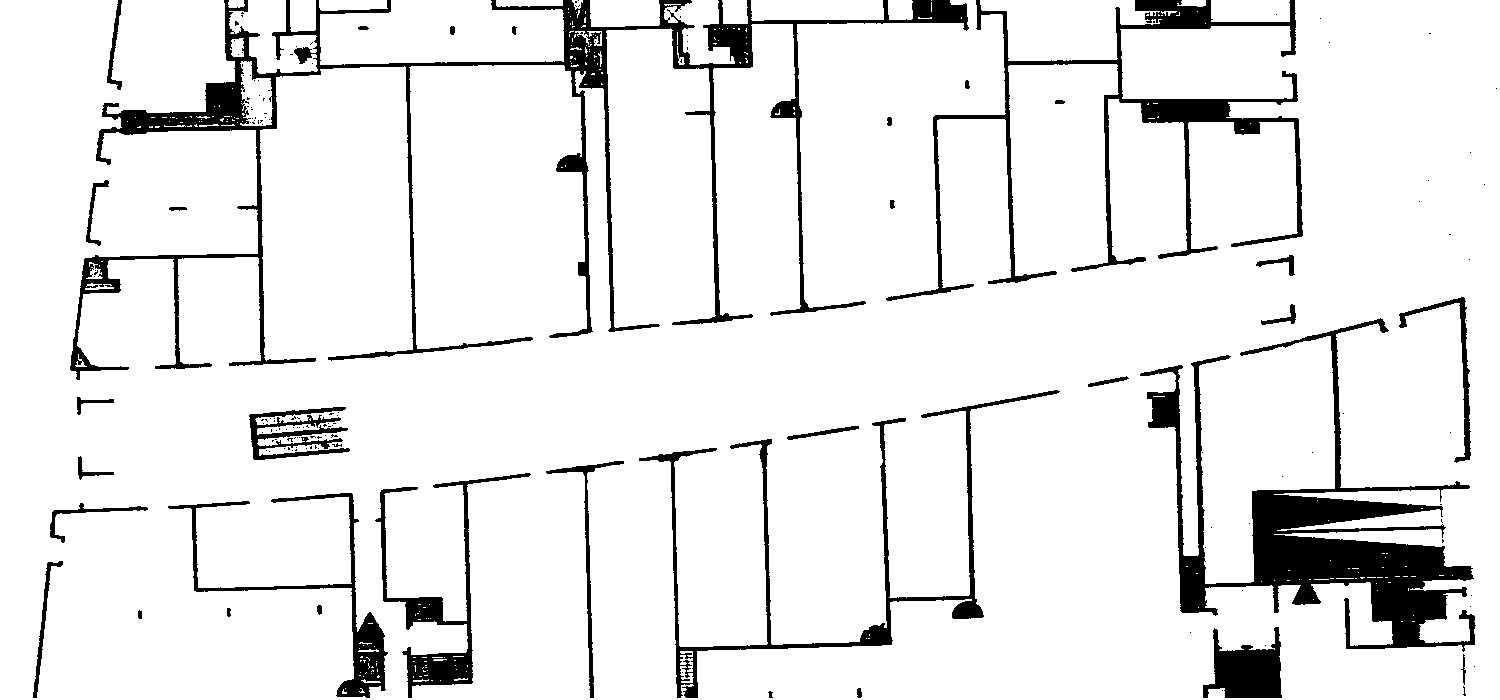
\includegraphics[width=0.95\textwidth]{Rive1.png}
\caption{2D map of the \emph{Rive de l'orne} shopping center.}
\label{fig:stage}
\end{figure}


In the Stage simulator the following map of the \emph{Rive de l'orne} shopping center has been realized. In Figure \ref{fig:stage} a section of the shopping mall in which we will deploy the prototypes is shown.
Additional maps have been realized for reproducing the environments of the partners in which some experiments will be performed.

The Stage environment models one or more robots that have the same 2D sensor and actuator configurations of the real ones and some additional mobile obstacles that represent people moving in the environment. Several behaviors can be tested in this simulated environment such as: 2D perception of human behaviors, human-robot social navigation (e.g., following a person or guiding a person), safe navigation in the environment.

The Stage environment has been fully realized and tested and this configuration will be used as a reference also for the development of the real robotic system.

\section{Data sets}

A number of data sets will be acquired in order to test sensor processing modules. In particular, data will be collected from laser range finder and RGBD cameras mounted on the robot in situations where people move around and approach the robot.

\begin{figure}
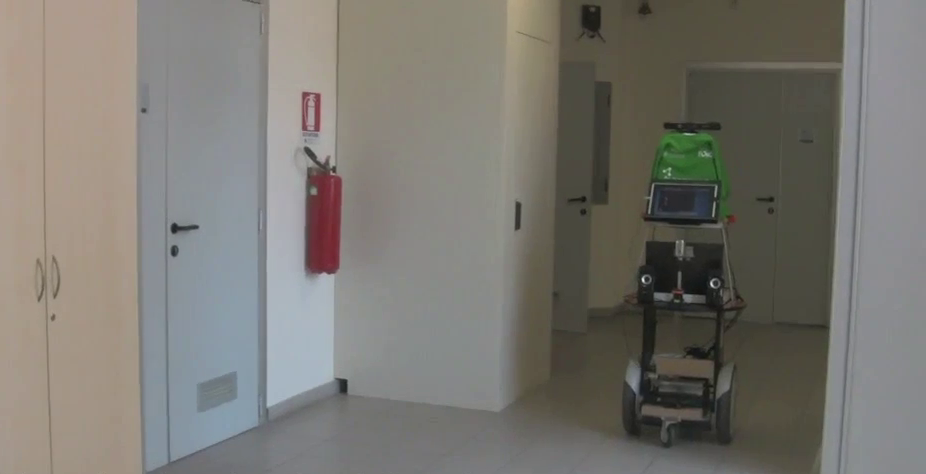
\includegraphics[width=0.95\textwidth]{diago.png}
\caption{Diago robot at Sapienza University of Rome.}
\label{fig:diago}
\end{figure}

In a first phase of the project,
the data sets have been captured with the mobile robot Diago in the Dept. of Computer, Control and Management Engineering, at Sapienza University of Rome (see Figure \ref{fig:diago}). Moreover, University of Caen will collect data in the same format with a similar robot in the \emph{Rive de l'orne} shopping mall.

The data sets specifications are given below.

\paragraph{Robot setup.} A robot moves in an environment populated by people. The robot is equipped with 1 laser and 1 (or more) RGBD camera and it is controlled by a human operator. The robot knows the map and it is localized in it at the beginning of the acquisition.

\paragraph{External camera setup (optional).}
One or more fixed cameras (either RGB or RGBD) is placed in the same environment as the robot and its position is registered in the world coordinates.

\paragraph{Acquisition.} On the robot(s) a ROS bag is acquired containing the following data (topics): 
TF, odom, cmd\_vel, stimated robot pose from localizer, laser and RBGD data. On the external camera(s) a video file. 

\paragraph{Data set.} The raw data streams acquired are processed in order to be easier to process. The resulting data set will contain:
\begin{itemize}
\item Robot Position: text file containing (timestamp, X, Y, THETA) (world coordinates)
\item Robot Laser: text file containing (timestamp, map$\langle$RHO, THETA$\rangle$)  (robot coordinates)
\item Robot Camera: image files:	(timestamp\_RGB.bmp or .jpg or .png) and
 				(timestamp\_DEPTH.png)
\item Camera: image files (as in the Robot Camera)
\end{itemize}

All time stamps must be synchronized. This synchronization will be performed at this stage by manually detecting and synchronizing a few corresponding frames in the different acquired data streams.

\paragraph{Ground-truth annotations.} The data set will be annotated in order to provide useful information for evaluating the processing algorithms.
The two elements annotated will be {\tt person}, representing an individual person in the scene, and {\tt group}, representing a group of people in the scene for which we are not interested in determining individuals.

For each person/group in the scene the following annotation will be used.

\begin{verbatim}
   <person id="..." timestamp="..." sensorid="...">
      <x> ... </x>
      <y> ... </y>
      <bbx> ... </bbx>
      <bby> ... </bby>
      <bbw> ... </bbw>
      <bbh> ... </bbh>
      <gender> ... </gender>
      <age> ... </age>
      <identity> ... </identity>
      <activity> ... </activity>
   </person> 
\end{verbatim}

\begin{verbatim}
   <group id="..." timestamp="..." sensorid="...">
      <x> ... </x>
      <y> ... </y>
      <bbx> ... </bbx>
      <bby> ... </bby>
      <bbw> ... </bbw>
      <bbh> ... </bbh>
      <size> ... </size>
      <activity> ... </activity>
   </group> 
\end{verbatim}

where:


\begin{verbatim}
      id: person or group id (unique anonymous identifier for every person/group appearing in the data set)
      timestamp: timestamp of reference
      sensorid: sensor with which the person/group has been detected
      x, y: floor projection of baricenter of the person/group (world coordinates)
      bbx, bby: coordinates of the top left point of the bounding box (image coordinates)
      bbw, bbh: width and height of the bounding box (image coordinates)
      gender: gender of person 
      age: age category (child, adult, senior)
      identity: the identity of the person (name, birth date, ...)
      size: number of people in the group
      activity: a set of symbols representing activities of the person/group
\end{verbatim}

An annotation is made every several frames (e.g., 60 frames or 5 seconds). {\tt id} of people and groups are maintained over different sensors and over time, even when the person/group move through different sensors.

Notice also that identity of people will be gathered and stored only for the people that are involved in the development of the project, who agree on this procedure and on the use of these information. In no case, these information will be collected from visitors or other users that are not involved with the partners of the project.
In some experiments, some invented identities will be associated to users. 

\section{Software organization and version management}

In order to manage the development of the software by all the partners of the project, we have supported the team from University of Caen in the set up of a GIT repository for the software.
The repository is accessible only by the project partners and it is organized as follows.

The 'coaches/software' folder contains source code, libraries and binary code 
divided in the following sub-folders:

\begin{itemize}
\item \emph{src}:       contains (non-ROS) source code maintained in the coaches repository
\item \emph{ros}:       contains ros modules
\item \emph{external}:  contains external software not maintained in the coaches repository
\item \emph{bin}:       contains executable files
\item \emph{include}:   contains include files 
\item \emph{lib}:       contains libraries
\end{itemize}


The \emph{ros} folder contains a Catkin workspace (which is the standard building environment in ROS) and the following ROS packages, including the robotic software components described above.

\begin{itemize}
\item \emph{hello\_coaches\_developers}: a test package to check correct installation and set-up of the environment;
\item \emph{t11\_kb\_modeling}: software developed for Task T1.1;
\item \emph{t12\_kb\_reasoning}: software developed for Task T1.2;
\item \emph{t21\_image\_processing}: software developed for Task T2.1;
\item \emph{t22\_situation\_awareness}: software developed for Task T2.2;
\item \emph{t31\_multimodal\_hri}: software developed for Task T3.1;
\item \emph{t32\_human\_needs\_estimation}: software developed for Task T3.2;
\item \emph{t41\_robust\_navigation}: software developed for Task T4.1;
\item \emph{t42\_multi\_robot\_planning}: software developed for Task T4.2;
\end{itemize}


Moreover, additional packages developed outside the COACHES project are present in the \emph{external} directory and linked in the ROS Catkin workspace.
Some examples of these external packages are:
\begin{itemize}
\item \emph{gradient\_based\_navigation}: a package for safe navigation and obstacle avoidance in dynamic environments;
\item \emph{PetriNetPlans}: library and ROS bridge for plan execution;
\item \emph{stage\_environments}: a package for 2D simulation.
\end{itemize}

Automated scripts for initializing, setting-up, updating, building and testing the software environment have been developed and described in the repository. These scripts facilitate updates and testing and thus in  general the integration of functionalities developed by the different developers.

\begin{itemize}
\item \emph{coaches\_init}: initialize the software development environment (to be run once in every computer used for development);
\item \emph{coaches\_setup}:   set up all the system variables needed for development (to be run on every shell used for development);
\item \emph{coaches\_update}:  update of all the software from the GIT repository to the local workspace;
\item \emph{coaches\_make}:   build all the software
\end{itemize}

\section{Test}

The software environment has been succesfully tested by different developers from different partners using different machines, including laptops running the software for the real robots.

\end{document}
